


\newpage
\appendix
\section*{Apéndice}

\section{Diagnóstico de Cáncer de Mama }
Este apéndice reúne todas las figuras y tablas incluidas a lo largo del análisis del Diagnóstico de Cáncer de Mama. Cada recurso visual o tabular se encuentra correctamente referenciado en el cuerpo principal, y aquí se presentan organizados para facilitar su consulta y comparación posterior.


\subsection{Modelado Predictivo}\label{subsec:modelado-predictivo}


El modelo utilizado fue regresión logística regularizada para clasificación binaria. La probabilidad de que una observación \(\mathbf{x}\) pertenezca a la clase positiva se modela mediante la función sigmoide:

\begin{equation}
P(y = 1 \mid \mathbf{x}) = \frac{1}{1 + e^{-(\beta_0 + \boldsymbol{\beta} \cdot \mathbf{x})}}.
\end{equation}

La función de pérdida base se define como la entropía cruzada:

\begin{equation}
\mathcal{L}(\boldsymbol{\beta}) = -\frac{1}{n} \sum_{i=1}^{n} \left[ y_i \log \hat{y}_i + (1 - y_i) \log(1 - \hat{y}_i) \right],
\end{equation}

donde \(\hat{y}_i = P(y_i = 1 \mid \mathbf{x}_i)\). Para mitigar el sobreajuste, se aplicó una penalización L2:

\begin{equation}
\mathcal{L}_{\text{reg}}(\boldsymbol{\beta}) = \mathcal{L}(\boldsymbol{\beta}) + \lambda \|\boldsymbol{\beta}\|_2^2.
\end{equation}

El modelo fue optimizado mediante descenso por gradiente, con una tasa de aprendizaje de 0.01, tolerancia de convergencia de \(1 \times 10^{-4}\) y un máximo de 1000 iteraciones.


\subsection{Manejo del Desbalanceo}\label{subsec:desbalanceo}

Dado el desbalance observado entre clases, se aplicaron cuatro estrategias de re-balanceo: \textit{undersampling}, \textit{oversampling}, \textit{SMOTE} y \textit{cost reweighting}. La Tabla~\ref{tab:rebalanceo} presenta la distribución de observaciones resultante para cada técnica.

La técnica de \textbf{undersampling} reduce aleatoriamente el número de observaciones de la clase mayoritaria hasta igualarlo con el de la clase minoritaria.

En \textbf{oversampling}, se replican aleatoriamente ejemplos de la clase minoritaria hasta igualar las cantidades entre clases.

\textbf{SMOTE} (Synthetic Minority Over-sampling Technique) genera nuevas instancias sintéticas de la clase minoritaria interpolando entre observaciones reales cercanas.

Por su parte, \textbf{cost reweighting} modifica la función de pérdida del modelo, penalizando con mayor intensidad los errores sobre la clase minoritaria. La función ajustada se define como:

\begin{equation}
\mathcal{L} = -\sum_{i=1}^{n} w_{y_i} \left[ y_i \log(\hat{y}_i) + (1 - y_i) \log(1 - \hat{y}_i) \right],
\end{equation}

donde los pesos de clase se fijan como \( w_0 = 1 \) y \( w_1 = \pi_2 / \pi_1 \), siendo \( \pi_1 \) y \( \pi_2 \) las proporciones de la clase minoritaria y mayoritaria, respectivamente.

Cada una de estas estrategias fue implementada por separado y evaluada en términos de su impacto sobre el rendimiento del modelo, con énfasis en su capacidad para detectar correctamente la clase positiva.




\subsection{Ajuste de Hiperparámetros}\label{subsec:hiperparams-cancer}

La validación cruzada se utilizó para ajustar el hiperparámetro de regularización \(\lambda\). Se exploró un rango logarítmico entre \(10^{-6}\) y \(10^1\). En todos los escenarios se mantuvo la misma configuración de entrenamiento, variando únicamente la estrategia de re-balanceo. Para el caso de datos balanceados, se obtuvo $\lambda= 10.0 $. Por otro lado, para el conjunto de datos desbalanceados, los valores óptimos obtenidos para cada técnica se resumen en la Tabla~\ref{tab:optimal_lambda}.




\subsection{Figuras}

A continuación se presentan las principales visualizaciones utilizadas en el desarrollo del informe. Las mismas se encuentran organizadas por temática: tratamiento de valores atípicos, análisis de distribuciones, y evaluación de modelos.

\subsubsection*{Evaluación de Modelos}

\begin{figure}[H]
    \centering
    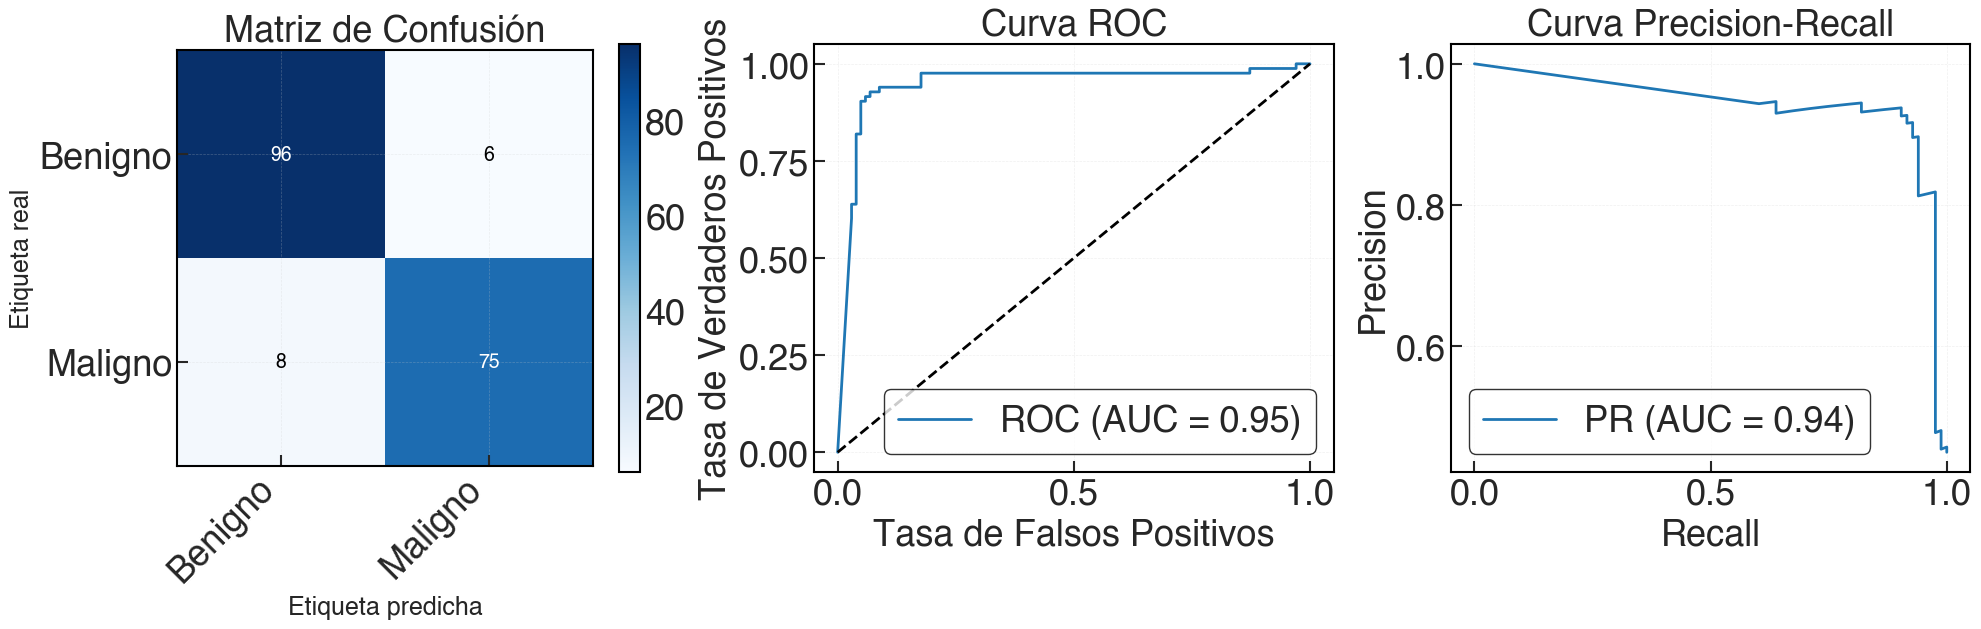
\includegraphics[width=0.8\linewidth]{figures/p1/roc_auc_balanced_test.png}
    \caption{Curva ROC del modelo entrenado sobre datos balanceados y evaluado en el conjunto de prueba.}
    \label{fig:roc_auc_balanced_test}
\end{figure}

\begin{figure}[H]
    \centering
    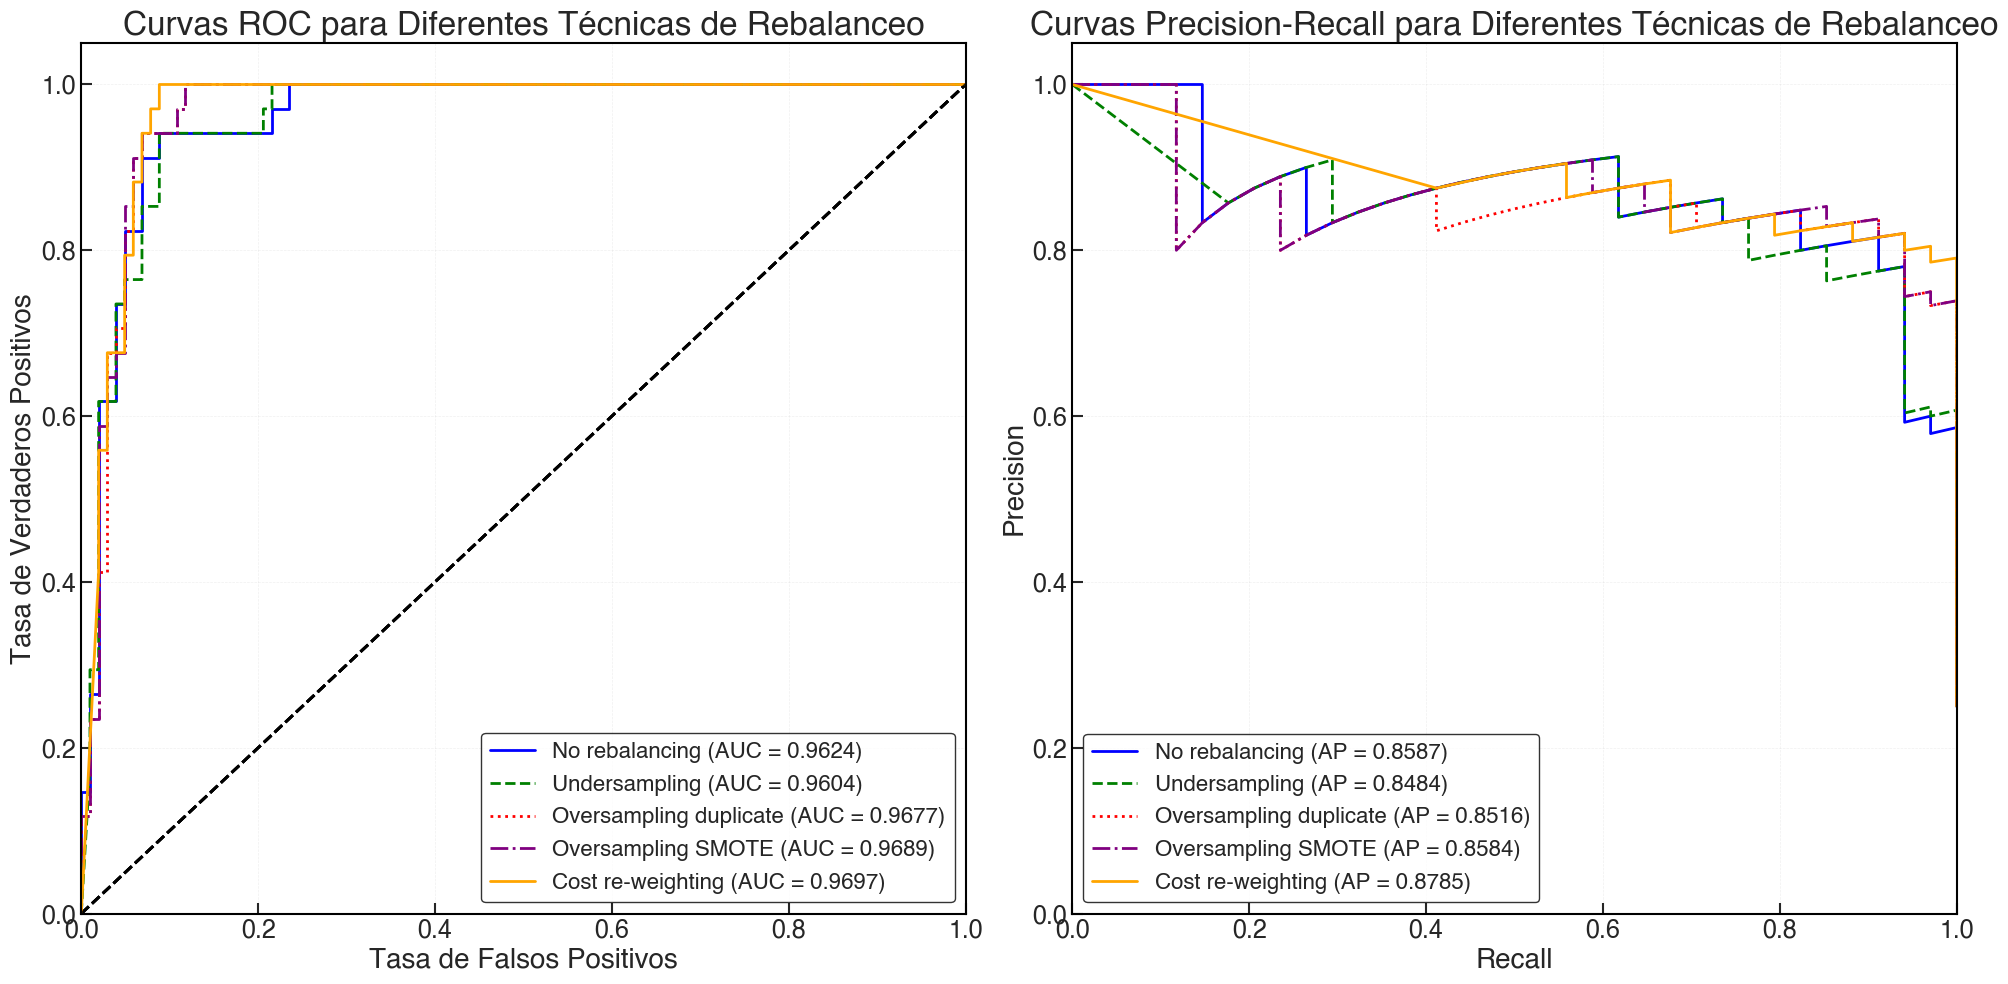
\includegraphics[width=0.8\linewidth]{figures/p1/roc_auc_imbalanced_test.png}
    \caption{Curvas ROC y PR de los modelos entrenados con distintas técnicas de rebalanceo (conjunto desbalanceado).}
    \label{fig:roc_auc_imbalanced_test}
\end{figure}

\begin{figure}[H]
    \centering
    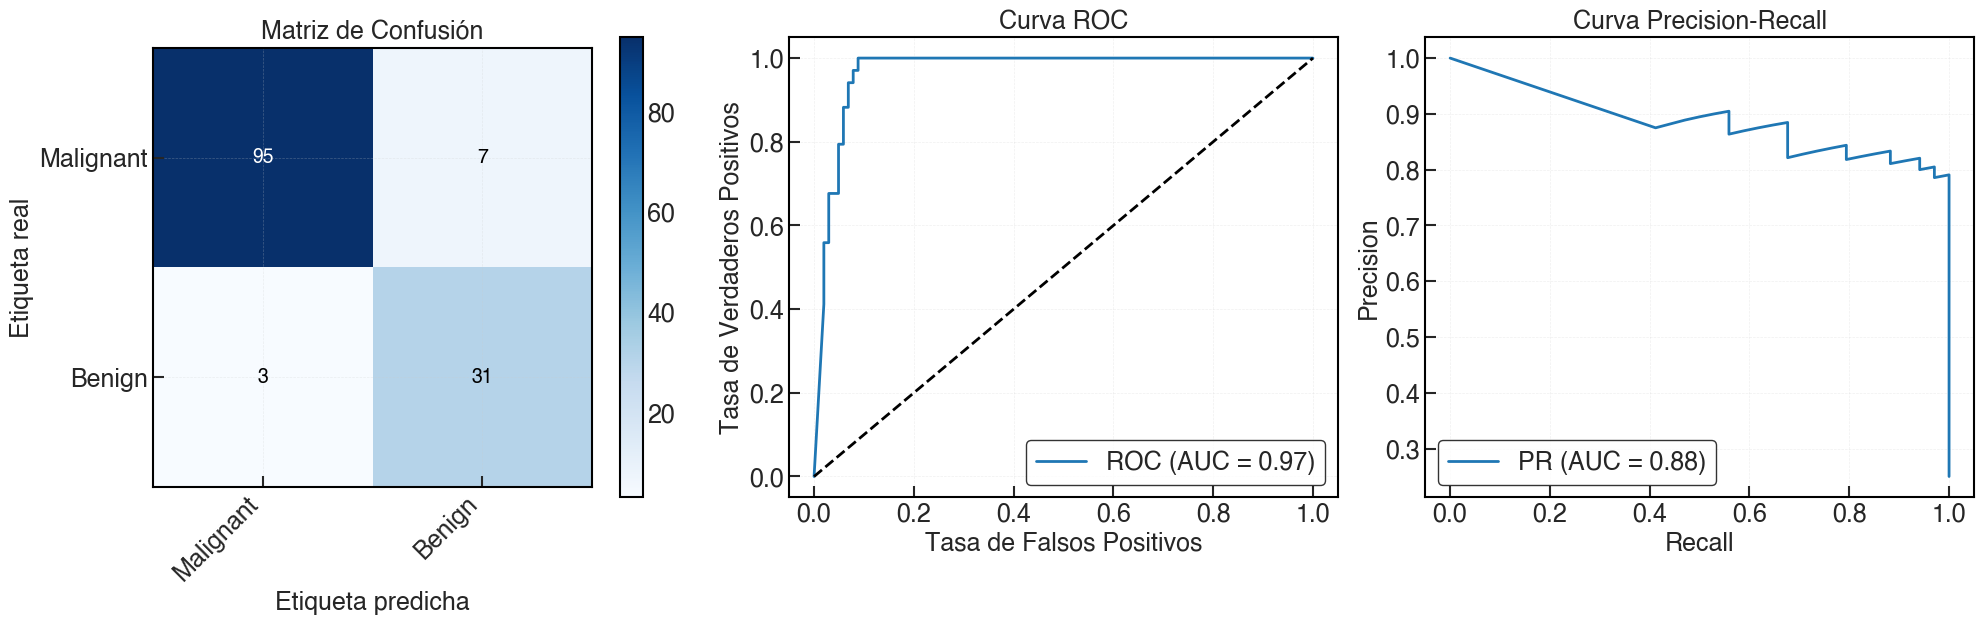
\includegraphics[width=0.8\linewidth]{figures/p1/metric_plot_imbalanced_cw.png}
    \caption{Resumen gráfico del modelo final entrenado con \textit{cost re-weighting}. Incluye matriz de confusión, curva ROC y curva PR.}
    \label{fig:metric_plot_imbalanced_cw}
\end{figure}


\subsection{Tablas}


\begin{table}[H]
\centering
\caption{Valores óptimos de \(\lambda\) por técnica de re-balanceo.}
\label{tab:optimal_lambda}
\begin{tabular}{lc}
\toprule
\textbf{Técnica de re-balanceo} & \textbf{Valor óptimo de \(\lambda\)} \\
\midrule
Sin re-balanceo        & 10 \\
Undersampling          & 1.27 \times 10^{-5} \\
Oversampling           & 0.78 \\
SMOTE                  & 4.28 \\
Cost reweighting       & 0.34 \\
\bottomrule
\end{tabular}
\end{table}

\begin{table}[H]
\centering
\caption{Técnicas de re-balanceo aplicadas y distribución/clasificación resultante.}
\label{tab:rebalanceo}
\begin{tabular}{lccc}
\toprule
\textbf{Técnica} & \textbf{Clase 0} & \textbf{Clase 1} & \textbf{Pesos} \\
\midrule
Sin re-balanceo       & 732 & 243 & -- \\
Undersampling         & 243 & 243 & -- \\
Oversampling          & 732 & 732 & -- \\
SMOTE                 & 732 & 732 & -- \\
Cost reweighting      & 732 & 243 & 1.0 (0) / 3.0 (1) \\
\bottomrule
\end{tabular}
\end{table}

\begin{table}[H]
\centering
\caption{Desempeño del modelo con datos balanceados en validación y prueba.}
\label{tab:metrics_balanced}
\begin{tabular}{lcc}
\toprule
\textbf{Métrica} & \textbf{Validación} & \textbf{Prueba} \\
\midrule
Accuracy  & 0.9066 & 0.9189 \\
Precision & 0.8815 & 0.9250 \\
Recall    & 0.8881 & 0.8916 \\
F1 Score  & 0.8848 & 0.9080 \\
\bottomrule
\end{tabular}
\end{table}

\begin{table}[H]
\centering
\caption{Resumen de métricas en validación para cada técnica de re-balanceo.}
\label{tab:val-metrics-imbalanced}
\begin{tabular}{lcccccc}
\toprule
\textbf{Técnica} & \textbf{Accuracy} & \textbf{Precision} & \textbf{Recall} & \textbf{F1-Score} & \textbf{AUC-ROC} & \textbf{AUC-PR} \\
\midrule
No rebalancing           & 0.9050 & 0.8136 & 0.8000 & 0.8067 & 0.9571 & 0.8468 \\
Undersampling            & 0.9132 & 0.8000 & 0.8667 & 0.8320 & 0.9584 & 0.8468 \\
Oversampling             & 0.8967 & 0.7465 & 0.8833 & 0.8092 & 0.9641 & 0.8676 \\
SMOTE                    & 0.9174 & 0.8030 & 0.8833 & 0.8413 & 0.9642 & 0.8654 \\
Cost re-weighting        & 0.9132 & 0.7910 & 0.8833 & 0.8346 & 0.9668 & 0.8819 \\
\bottomrule
\end{tabular}
\end{table}

\begin{table}[H]
\centering
\caption{Resumen de métricas en el conjunto de prueba para cada técnica de re-balanceo.}
\label{tab:test-metrics-imbalanced}
\begin{tabular}{lcccccc}
\toprule
\textbf{Técnica} & \textbf{Accuracy} & \textbf{Precision} & \textbf{Recall} & \textbf{F1-Score} & \textbf{AUC-ROC} & \textbf{AUC-PR} \\
\midrule
No rebalancing           & 0.9044 & 0.8621 & 0.7353 & 0.7937 & 0.9624 & 0.8587 \\
Undersampling            & 0.9044 & 0.8387 & 0.7647 & 0.8000 & 0.9604 & 0.8484 \\
Oversampling             & 0.9338 & 0.8378 & 0.9118 & 0.8732 & 0.9677 & 0.8516 \\
SMOTE                    & 0.9265 & 0.8529 & 0.8529 & 0.8529 & 0.9689 & 0.8584 \\
Cost re-weighting        & 0.9265 & 0.8158 & 0.9118 & 0.8611 & 0.9697 & 0.8785 \\
\bottomrule
\end{tabular}
\end{table}




\section{Clasificación de Jugadores de Baloncesto}


Este apéndice reúne todas las figuras y tablas incluidas a lo largo del análisis de la Clasificación de Jugadores de Baloncesto. Cada recurso visual o tabular se encuentra correctamente referenciado en el cuerpo principal, y aquí se presentan organizados para facilitar su consulta y comparación posterior.



\subsection{Modelado Predictivo}\label{subsec:modelado-predictivo-p2}


Para abordar la tarea de clasificación, se implementaron distintos enfoques de modelado supervisado, evaluando sus capacidades predictivas sobre el conjunto de datos procesado.

\subsubsection{Regresión Logística Multiclase}
La regresión logística multiclase utiliza la función softmax para modelar la probabilidad de clase:

\begin{equation}
P(y = k \mid \mathbf{x}) = \frac{e^{\beta_0^{(k)} + \boldsymbol{\beta}^{(k)} \cdot \mathbf{x}}}{\sum_{j=1}^{K} e^{\beta_0^{(j)} + \boldsymbol{\beta}^{(j)} \cdot \mathbf{x}}}.
\end{equation}

La función de pérdida sin regularización es la entropía cruzada:

\begin{equation}
\mathcal{L}(\boldsymbol{\beta}) = -\frac{1}{n} \sum_{i=1}^{n} \sum_{k=1}^{K} \mathbb{1}(y_i = k) \log P(y_i = k \mid \mathbf{x}_i),
\end{equation}

y su versión regularizada con penalización L2 es:

\begin{equation}
\mathcal{L}_{\text{reg}}(\boldsymbol{\beta}) = \mathcal{L}(\boldsymbol{\beta}) + \lambda \sum_{k=1}^{K} \|\boldsymbol{\beta}^{(k)}\|_2^2.
\end{equation}

La calibración del parámetro de regularización \(\lambda\) se realizó mediante validación cruzada estratificada (5 folds), explorando un rango logarítmico entre \(10^{-6}\) y \(10^1\). Se eligió como métrica de evaluación el F1-score ponderado, y se obtuvo un valor óptimo de \(\lambda = 10\). Además, el modelo fue entrenado con los datos normalizados con el fin de garantizar que todas las variables numéricas tuvieran la misma escala, lo cual resulta fundamental para evitar sesgos en el proceso de optimización y asegurar una correcta convergencia del algoritmo de descenso por gradiente.

\subsubsection{Análisis Discriminante Lineal (LDA)}

El modelo LDA asume que cada clase se distribuye según una normal multivariada con media \(\boldsymbol{\mu}_c\) y covarianza común \(\boldsymbol{\Sigma}\). Es por esto que el modelo utilizado fue entrenado con los datos normalizados. La función discriminante es:

\begin{equation}
\delta_c(\mathbf{x}) = \gamma_c + \boldsymbol{\beta}_c^\top \mathbf{x},
\end{equation}

donde

\begin{equation}
\boldsymbol{\beta}_c = \boldsymbol{\Sigma}^{-1} \boldsymbol{\mu}_c, \quad
\gamma_c = \log \pi_c - \frac{1}{2} \boldsymbol{\mu}_c^\top \boldsymbol{\Sigma}^{-1} \boldsymbol{\mu}_c.
\end{equation}

La clase predicha es la que maximiza \(\delta_c(\mathbf{x})\). Para obtener probabilidades predictivas, se aplica una normalización tipo softmax.


\subsubsection{Random Forest}

El modelo Random Forest se construyó como un conjunto de árboles entrenados sobre subconjuntos \textit{bootstrap}. En cada nodo, se eligió el umbral que maximizó la ganancia de información:

\begin{equation}
\mathrm{IG} = \mathcal{I}(y) - \frac{m_L}{m}\mathcal{I}(y_L) - \frac{m_R}{m}\mathcal{I}(y_R),
\end{equation}

donde \(\mathcal{I}\) representa la entropía. La predicción final del modelo se obtuvo mediante votación mayoritaria:

\begin{equation}
\hat{y} = \mathrm{mode}(h_1(x), h_2(x), \dots, h_T(x)).
\end{equation}

Se utilizó una configuración compacta: tres árboles con profundidad máxima 10, al menos dos muestras por nodo y una por hoja. Se seleccionaron atributos al azar (\texttt{sqrt} del total) y se usó entropía como criterio de división.



\subsection{Figuras}



\begin{figure}[H]
    \centering
    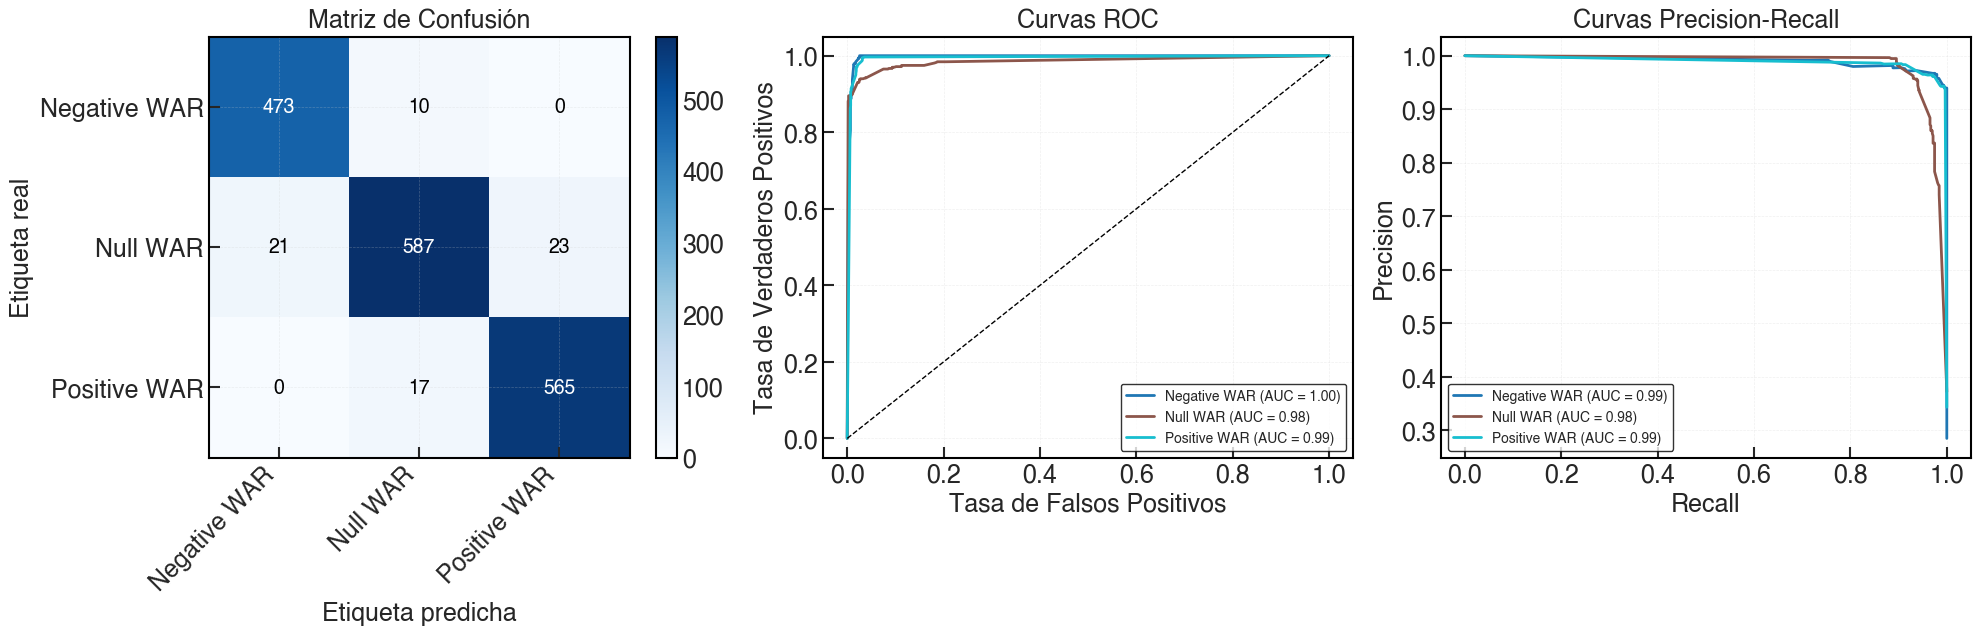
\includegraphics[width=0.8\linewidth]{figures//p2/roc_pr_random_forest_test.png}
    \caption{Resumen gráfico de métricas del modelo entrenado con Random Forest y evaluado sobre el conjunto de prueba.}
    \label{fig:roc_pr_random_forest_test}
\end{figure}


\subsection{Tablas}


\begin{table}[H]
\centering
\caption{Desempeño de modelos sobre el conjunto de prueba \texttt{WAR\_class\_test} }
\label{tab:metrics_war_class}
\begin{tabular}{lcccc}
\toprule
\textbf{Modelo} & \textbf{Accuracy} & \textbf{Precision} & \textbf{Recall} & \textbf{F1 Score} \\
\midrule
Regresión Logística Multiclase & 0.8874 & 0.8956 & 0.8874 & 0.8836 \\
LDA (solver='svd') & 0.9051 & 0.9145 & 0.9051 & 0.9020 \\
Random Forest (T=3) & \textbf{0.9581} & \textbf{0.9581} & \textbf{0.9581} & \textbf{0.9580} \\
\bottomrule
\end{tabular}
\end{table}

\begin{table}[H]
\centering
\caption{Desempeño de modelos sobre el conjunto de validación}
\label{tab:val_war_class}
\begin{tabular}{lcccc}
\toprule
\textbf{Modelo} & \textbf{Accuracy} & \textbf{Precision} & \textbf{Recall} & \textbf{F1 Score} \\
\midrule
Regresión Logística Multiclase & 0.6041 & 0.4218 & 0.6041 & 0.4965 \\
LDA (solver='svd') & 0.9232 & 0.9322 & 0.9232 & 0.9215 \\
Random Forest (T=3) & \textbf{0.9845} & \textbf{0.9847} & \textbf{0.9845} & \textbf{0.9845} \\
\bottomrule
\end{tabular}
\end{table}


\section{Imputación con KNN}
\label{subsec:knn}

Para el tratamiento de valores faltantes en variables numéricas, se utilizó el algoritmo \textit{K-Nearest Neighbors} (KNN). Este método imputa valores ausentes en función de las observaciones más similares (vecinas), calculadas mediante una métrica de distancia. En este trabajo, se empleó la distancia euclidiana:

\begin{equation}
d(\mathbf{x}, \mathbf{y}) = \sqrt{\sum_{i=1}^{n} (x_i - y_i)^2},
\end{equation}

donde \(\mathbf{x}\) y \(\mathbf{y}\) son vectores de características de dos observaciones, e \(n\) representa el número de atributos considerados. 


% Descripción del procedimiento KNN

\section{Winsorización por IQR}
\label{subsec:iqr}



Los valores atípicos fueron identificados mediante el método del rango intercuartílico (IQR), una técnica robusta basada en estadísticos de posición. Dado un conjunto de datos, se calcularon los cuartiles \(Q_1\) (percentil 25) y \(Q_3\) (percentil 75), definiendo el IQR como:

\begin{equation}
IQR = Q_3 - Q_1.
\end{equation}

Los umbrales para considerar un valor como atípico fueron:

\begin{equation}
L_{\text{inf}} = Q_1 - 1.5 \times IQR, \quad L_{\text{sup}} = Q_3 + 1.5 \times IQR.
\end{equation}

Los valores fuera de este rango fueron considerados outliers y tratados mediante winsorización, es decir, se truncaron al valor del límite más próximo (\(L_{\text{inf}}\) o \(L_{\text{sup}}\)). Esta técnica conserva todas las observaciones, pero limita el impacto de valores extremos sobre el modelo, estabilizando las distribuciones sin alterar la cantidad de datos disponibles.

Este procedimiento fue aplicado a todas las variables numéricas clave antes del entrenamiento de modelos predictivos.




\section{Métricas de Desempeño}\label{subsec:metricas-desempenio}

Para medir el rendimiento, se emplearon las métricas clásicas de clasificación: precisión, recall, F1-score, exactitud, AUC-ROC y AUC-PR. La precisión se define como:

\begin{equation}
\text{Precision} = \frac{TP}{TP + FP},
\end{equation}

el recall como:

\begin{equation}
\text{Recall} = \frac{TP}{TP + FN},
\end{equation}

el F1-score como:

\begin{equation}
F1 = 2 \cdot \frac{\text{Precision} \cdot \text{Recall}}{\text{Precision} + \text{Recall}},
\end{equation}

y la exactitud como:

\begin{equation}
\text{Accuracy} = \frac{TP + TN}{TP + TN + FP + FN}.
\end{equation}

Las curvas ROC y PR fueron construidas variando el umbral de decisión. Las áreas bajo dichas curvas (AUC) se utilizaron como indicadores de desempeño global.

